\chapter{Anatomical Region Prior Model}
\label{ch:new_model}
%


When considering using more than one data modality for analysis, there are many ways to combine them. 
%
The asymmetric multi-modal data analysis paradigm consists of selecting a tool designed for one data modality and then incorporating information from all the other data modalities into the analysis.
%
This paradigm fits the purpose of performing the Electronic Source Imaging while incorporating information from additional data modalities.

%Within the asymmetric multi-modal data analysis paradigm, we aim to enhance the ESI data by incorporating information from other measurement modalities.

In particular, we consider the case in which a physical region is known to produce a higher background electrical activity.
%
The location and extent of this region are observed using some imaging techniques independent of EEG.

The motivation for this particular setup comes from a specific experimental setup in which an ischemic stroke is induced, and later, the affected area is determined using histochemical analysis.

\section{Model Assumptions}

The relationship between the recordings from surface electrodes, $\Y$, and the magnitudes of equivalent distributed dipoles located inside the brain, $\SA$, is given by the following equation
\begin{equation}
\Y = \G \ppar{\SA + \varepsilon},
\label{eq:3.1}
\end{equation}
with $\Y \in \R^{M \times 1}$, $\SA \in \R^{3N \times 1}$, $\G \in \R^{3N\times M}$, and $\varepsilon\in \R^{N\times 1}$.
%
This model was described in detail in Chapter \ref{ch:forward}, including the interpretation and derivation of the leadfield matrix $\G$.
%
Notice that this model considers only internal noise.

Ideally, the extra information provided by the additional data modality should allow us to identify an anatomical region exhibiting pathological behavior; for simplicity, we refer to this region as a P-region. 
%
For generality, we consider the possibility of multiple disjoint P-regions, say $K$ with $1\leq K < \infty$.
%
P-regions are labeled $P_1, P_2, \dots, P_K$, with $P_0$ the dipoles outside all P-regions.
%
For notation, define 
\begin{equation}
    P_k = \sset{ n\in \sset{1, 2, \dots, N} \given n\text{-th dipole is in the } k\text{-th region} }
\end{equation}

\begin{figure}
    \centering 
    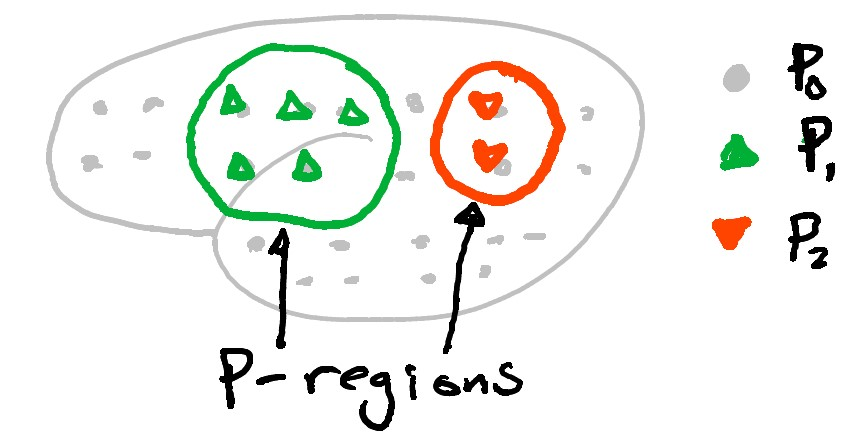
\includegraphics[width=0.6\linewidth]{./img_dev/Pregions.jpg}
    \caption{Construction of labels based on P-regions, representing regions when a particular symptom, independent of electrophysiological measurements, was observed.}
\end{figure}

As a remark, the P-regions are defined independently of the dipoles; each $P_k$ is the set of dipoles inside a specific P-region.

For ease of handling in the model, the P-regions regions are encoded using the matrix 
$\PA\in \sset{0,1}^{N\times K}$ defined as
\begin{equation}
    \PA\ppar{n,k} = \begin{cases}
        1, &\text{if } n \in P_k \\
        0, &\text{otherwise.}
    \end{cases}
\end{equation}

In section \ref{sec:SelectPregions}, we describe heuristic methods to determine the P-regions and, consequently, the matrix $\PA$.

%The P-region is encoded into the model as a labeling variable 
%${Z\in \sset{0,1}^{N\times 1}}$, so that $Z_n = 1$ if the $n$-th dipole is located on a the active region.

%\begin{figure}
%\centering
%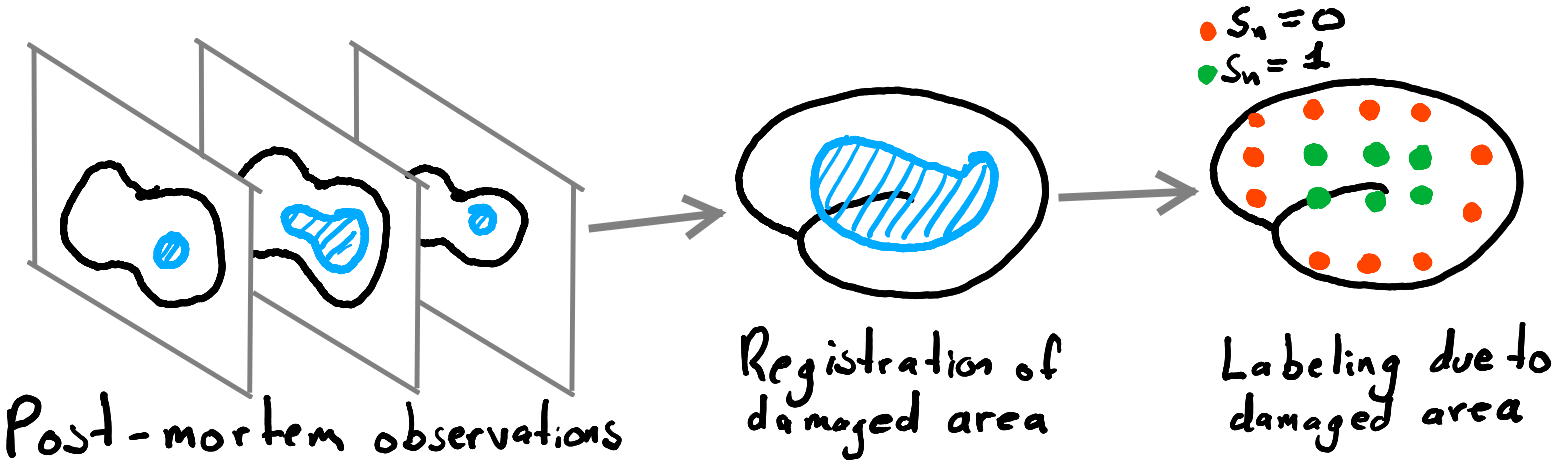
\includegraphics[width=0.8\linewidth]{./img/sketch02_v2}
%\end{figure}

The relation between the current density, $\SA$, and the P-regions is incorporated into the model by adjusting the covariance of $\SA$ depending on which P-region it is located.
%
To be specific, consider,
\begin{equation}
    \ccov{\SA\ppar{n_1}, \SA\ppar{n_2}} = 
    \begin{cases}
        \gamma_k, & \text{if } n_1, n_2\in P_k, \\
        0, & \text{otherwise}
    \end{cases}
\end{equation}
with $0 < \gamma_0 \ll \gamma_k$ for $1\leq k \leq K$.
%
This guarantees that P-regions have synchronized activity that is larger in magnitude than the background activity.

The assumption of a perfect synchrony is introduced in order to simplify the model.
%
We can separate the source, $\SA$, into a regionally-synchronized activity, $\RA$, and a background noise, $\BA$, as
\begin{equation}
    \SA +\varepsilon = \BA + \PA \RA = \BA + \sum_{k=1}^K \PA(:,k)\, \RA(k)
    \label{eq:3.4}
\end{equation}
with $\BA \in \R^{N\times 1}, \RA \in \R^{K\times 1}$ independent with each other.
%
These assumptions about P-regions can be combined with Gaussian assumptions, leading to 
\begin{align}
    \BA &\sim \norm\ppar{0, \gamma_0 \id_N } 
    \label{eq:3.5} \\
    \RA &\sim \norm\ppar{0, 
    \spar{\text{diag}\ppar{\gamma_1, \gamma_2, \dots, \gamma_K}-\gamma_0 \id_K} }
    \label{eq:3.6}
\end{align}

%%%%%%%%%%%%%%%%%%%%%%%%%%%%%%%%%%%%%%%%%%%%%%%%%%%%%%%%%%%%%%%%%%%%%%%%

\section{Proposed Estimator}

Given the assumptions described in the previous section, we propose constructing a linear estimator for $S$ similar to those presented in Chapter \ref{ch:review}.
%
%This choice follows the analysis of strengths and weaknesses. 
%
This choice follows the expectation of short computation times and memory requirements. 
%
We expect that the additional information from P-regions will decrease spatial dispersion while not significantly increasing computational speed.


The estimator of $\SA$ will be constructed as a Maximum A Posteriori estimator, maximizing the log probability of $\left. \SA \given \Y \right.$, as
\begin{align}
    \hat{\SA} &= 
    \argmax_{\SA }\, 
    \phantom{.}
    \log\ppar{
    \text{Prob}\ppar{ \SA \given \Y }}
    \nonumber \\
    &=
    \argmax_{\SA }\, 
    \phantom{.}
    \log \ppar{
    \text{Prob}\ppar{ \Y \given \SA }\,  \text{Prob}\ppar{ \SA } }
\end{align}
the structure of P-regions is incorporated by using the following decomposition
\begin{equation}
    {\SA} = {\BA} + \PA {\RA}
    = {\BA} + \sum_{k=1}^K \PA(:,k) {\RA}(k)
    \label{eq:3.7_v2}
\end{equation}
and the model equation $\Y = \G \SA$ is incorporated as a constraint, resulting in the following optimization problem
\begin{align}
    \sset{ \hat{\BA}, \hat{\RA} } 
    =
    \argmax_{\BA, \RA }\, 
    &\phantom{.}
    \frac{\sigma}{2 \gamma_0} \nnorm{\BA}^2
    +
    \sum_{k=1}^K \frac{\sigma}{2\ppar{\gamma_0-\gamma_k} } \nnorm{\PA(:,k)\, \RA(k)}^2
    \nonumber \\
    \text{s.t.}
    \quad
    &\phantom{.}
    {\G \ppar{\BA + \PA \RA} } - \Y = 0
    \label{eq:3.7}
\end{align}
where $\gamma_0, \gamma_1, \dots, \gamma_k, \sigma \in \R_+$ are parameters related to the assumed distributions of $\BA$ and $\SA$ given in equations \eqref{eq:3.5} and \eqref{eq:3.6}.
%
For ease of notation, we define the following equivalent parameters
\begin{align}
    \theta_0 &= \frac{1}{\sigma} \gamma_0 \\
    \theta_k &= \frac{1}{\sigma} \ppar{ \gamma_k- \gamma_0 },
    \text{ for } k = 1, 2, \dots, K.
\end{align}

Notice that the parameter $\sigma$ scales all the other parameters $\gamma_k$ equally, and thus, it can be ignored when discussing their relative magnitudes only.

%A careful derivation will reveal that $\theta_0 = \frac{\gamma_0 }{\sigma}$ and $\theta_k = \frac{\gamma_k-\gamma_0}{\sigma}$, with $\sigma>0$ the variance of the external noise.
%
%However, we decided that the role of those parameters within the interpretability of the model is negligible; we use $\theta_k$ as generic parameters that need to be tuned using the heuristics discussed in Chapter 2.

The constrained optimization problem in equation \eqref{eq:3.7} is solved using the method Lagrange multipliers.
%
First, we construct the respective Lagrangian function
\begin{align}
    \mathcal{L}\ppar{\BA, \RA, \lambda} &=
    \frac{1}{2 \theta_0} \nnorm{\BA}^2
    +
    \sum_{k=1}^K \frac{1}{2 \theta_k} \nnorm{\PA(:,k)\, \RA(k)}^2
    +
    \lambda^T \ppar{{\G \ppar{\BA + \PA \RA} } - \Y}
\end{align}
which can be minimized by solving the normal equations, i.e., the partial derivatives equal to zero.
%
The partial derivatives are given by
\begin{align}
    \frac{\partial}{\partial \BA} \mathcal{L}\ppar{\BA, \RA, \lambda}
    &=
    \frac{1}{\theta_0} \BA + \G^T \lambda 
    \label{eq:3.9}
    \\
    \frac{\partial}{\partial \RA(k)} \mathcal{L}\ppar{\BA, \RA, \lambda}
    &=
    \frac{1}{\theta_k} \PA(:,k)^T \PA(:,k)\, \RA(k) + \PA(:,k)^T \G^T \lambda 
    \label{eq:3.10}
    \\
    \frac{\partial}{\partial \lambda} \mathcal{L}\ppar{\BA, \RA, \lambda}
    &=
    \G \ppar{ \BA + \PA \RA } - \Y
    \label{eq:3.11}
\end{align}

Solving the normal equation for \eqref{eq:3.9} and \eqref{eq:3.10} lead to the following identities
\begin{align}
    \BA &= -\theta_0 \G^T \lambda
    \label{eq:3.13}
    \\
    \RA(k)
    &=
    -\theta_k \spar{\PA(:,k)^T \PA(:,k)}^{-1} \PA(:,k)^T \G^T \lambda 
    \label{eq:3.14}
\end{align}

Notice that $\PA(:,k)^T \PA(:,k) \in \mathbb{N}^{1\times 1}$ represents the number of dipoles on the $k$-th P-region, and thus is invertible.
%
For ease of notation, define
\begin{equation}
    \abss{P_k} = \PA(:,k)^T \PA(:,k)
\end{equation}

From equation \eqref{eq:3.11}, we may obtain a closed-form expression for $\lambda$,
\begin{align}
    \Y
    &=
    \G \BA + \G { \sum_{k=1}^K { \PA(:,k)\, \RA(k) } }
    \nonumber \\
    &=
    \G\ppar{-\theta_0 \G^T \lambda}
    + \G \sum_{k=1}^K
    { \PA(:,k)\, \ppar{-\theta_k \abss{P_k}^{-1} \PA(:,k)^T \G^T \lambda}}
    \nonumber \\
    &=
    -\G \ppar{ \theta_0 \id_N + \sum_{k=1}^K \theta_k \abss{P_k}^{-1} 
    \PA(:,k)\, \PA(:,k)^T
    } \G^T \lambda
\end{align}
which leads to the following identity
\begin{equation}
    \lambda
    =
    -\spar{\G \ppar{ \theta_0 \id_N + \sum_{k=1}^K \theta_k \abss{P_k}^{-1} 
    \PA(:,k)\, \PA(:,k)^T
    } \G^T}^{-1} \Y
\end{equation}

For robustness and to ensure that the resulting matrices are invertible, we propose using a regularized $\lambda_\rho$, defined as
%\begin{equation}
%    \lambda_\rho
%    =
%    -\spar{\G \ppar{ \theta_0 \id_N + \sum_{k=1}^K \theta_k \abss{P_k}^{-1} 
%    \PA(:,k)\, \PA(:,k)^T
%    } \G^T + \rho \id_M }^{-1} \Y
%\end{equation}
%and for a further simplification of notation, define
\begin{align}
    \lambda_\rho &= -W_\rho  \Y 
    \\
    W_\rho &=
    \spar{\G \ppar{ \theta_0 \id_N + \sum_{k=1}^K \theta_k \abss{P_k}^{-1} 
    \PA(:,k)\, \PA(:,k)^T
    } \G^T + \rho \id_M }^{-1}
\end{align}
where $\rho>0$ is a regularization parameter which must be determined using any of the heuristics defined in Chapter \ref{ch:review}.

Using $\lambda_\rho$ in equations \eqref{eq:3.13} and \eqref{eq:3.14} lead to the estimators
\begin{align}
    \hat{\BA} &=
    \theta_0 \G^T W_\rho \Y
    \\
    \hat{\RA}(k) &=
    \theta_k \abss{P_k}^{-1} \PA(:,k)^T \G^T W_\rho \Y
\end{align}

The estimator for $\SA$ is constructed as in equation \eqref{eq:3.7_v2},
\begin{align}
    \hat{\SA}
    &=
    \hat{\BA} + \sum_{k=1}^K \PA(:,k) \hat{\RA}(k)
    \nonumber \\
    &=
    \ppar{\theta_0 \G^T W_\rho \Y}
    + \sum_{k=1}^K \PA(:,k) \ppar{\theta_k \abss{P_k}^{-1} \PA(:,k)^T \G^T W_\rho \Y}
    \nonumber \\
    &=
    \ppar{ \theta_0 \id_N + \sum_{k=1}^K \theta_k \abss{P_k}^{-1} 
    \PA(:,k)\, \PA(:,k)^T
    } \G^T W_\rho \Y
\end{align}

Thus, the proposed estimator is given by
\begin{align}
    \hat{\SA}
    &=
    \ppar{ \theta_0 \id_N + \sum_{k=1}^K \theta_k \abss{P_k}^{-1} 
    \PA(:,k)\, \PA(:,k)^T
    } \G^T W_\rho \Y
    \label{eq:3.24}
    \\
    W_\rho &=
    \spar{\G \ppar{ \theta_0 \id_N + \sum_{k=1}^K \theta_k \abss{P_k}^{-1} 
    \PA(:,k)\, \PA(:,k)^T
    } \G^T + \rho \id_M }^{-1}
    \label{eq:3.25}
\end{align}

\subsection{Implementation notes}

The computation of the estimator described in equations \eqref{eq:3.24} and \eqref{eq:3.25} can be accelerated by avoiding explicit matrix multiplications whenever possible.
%
For instance, consider the matrices in the form 
\begin{equation}
    A_k = \abss{P_k}^{-1} \PA(:,k)\, \PA(:,k)^T
\end{equation}
for $1\leq k \leq K$. 
%
Notice that each $A_k \in \R^{N\times N}$ is an averaging operator with support over the corresponding P-region.
%
In other words, for any vector $V\in \R^{N}$ we have
\begin{equation}
    \spar{A_k V}(n) =
    \begin{cases}
        {\displaystyle \frac{1}{\abss{P_k}} \sum_{n'\in P_k} V(n')}, 
        &\text{if } n\in P_k, \\
        0, &\text{otherwise}.
    \end{cases}
\end{equation}

With this notation at hand, we can rewrite equation \eqref{eq:3.24} as
\begin{align}
    \hat{\SA}
    &=
    \ppar{\theta_0 \id_N + \sum_{k=1}^K \theta_k A_k}\G^T W_\rho \Y
\end{align}

%Instead of constructing the matrix $\ppar{\theta_0 \id_N + \sum_{k=1}^K \theta_k A_k}$ explicitly 

Using the matrices $A_k$, we can construct $\hat{\SA}$ row-by-row as follows:
\begin{align}
    \hat{\BA}_0
    &=
    \G^T W_\rho \Y \\
    \hat{\RA}_0(k)
    &=
    {\displaystyle \frac{1}{\abss{P_k}} \sum_{n\in P_k} \hat{\BA}_0(n)},
    \text{for } 1\leq k \leq K
    \\
    \hat{\SA}
    &=
    \theta_0 \hat{\BA}_0 + 
    \sum_{k=1}^K
    \theta_k \G\, \hat{\RA}_0(k)
    \label{eq:3.s1}
\end{align}
with $\hat{\BA}_0 \in \R^{N\times 1}$, $\hat{\RA}_0 \in \R^{K\times 1}$.
%
Alternatively, we can construct $\hat{\SA}$ row by row as
\begin{equation}
    \hat{\SA}(n) =
    \begin{cases}
        \theta_0 \hat{\BA}_0(n) + \theta_k \hat{\RA}_0(k),
        &\text{if } n\in P_k \text{ with } 1\leq k \leq K,
        \\
        \theta_0 \hat{\BA}_0(n), &\text{if } n\in P_0
    \end{cases}
    \label{eq:3.s2}
\end{equation}
Depending on how large the P-regions are, i.e., how large are each $\abss{P_k}$ with respect to $N$, it would be more convenient to use
either \eqref{eq:3.s1} or \eqref{eq:3.s2}.
%
In a practical setting, we informally expect each P-region to contain less than 10\% of the total dipoles.

%%%

Next, equation \eqref{eq:3.25} is simplified by considering the properties of the matrices involved.
%
Notice that each matrix $A_k$ is symmetric and idempotent.
%
Furthermore, if the P-regions are non-intersecting, then
\begin{equation}
    A_{k_1} A_{k_2} = 
    \begin{cases}
        A_{k_1}, &\text{if } k_1=k_2, \\
        0, &\text{otherwise.}
    \end{cases}
    \label{eq:3.27}
\end{equation}

This property can be extended to get powers and decomposition of the averaging operators $A_k$.
%
In particular, we have the following
\begin{equation}
    \ppar{q_0 \id_N + \sum_{k=1}^K q_k A_k}^2
    =
    q_0^2 \id_N + \sum_{k=1}^K \ppar{2q_0 q_k + q_k^2} A_k
\end{equation}
which leads to the following identity
\begin{align}
    \AAA_{\Theta} &=
    \sqrt{\theta_0} \id_N + \sum_{k=1}^K \ppar{\sqrt{\theta_0+\theta_k}-\sqrt{\theta_0}} A_k
    \\
    \AAA_{\Theta}^2
    &=
    {\theta_0} \id_N + \sum_{k=1}^K {\theta_k} A_k
\end{align}

With this decomposition at hand, we can rewrite $W_\rho$ as
\begin{equation}
    W_\rho =
    \spar{ \ppar{\G \AAA_{{\Theta}}} \ppar{\G \AAA_{{\Theta}}}^T
    + \rho \id_M }^{-1}
\end{equation}

Notice that $\AAA_\Theta\in \R^{N\times N}$ acts as a weighted average estimator over the rows of $\G$, a phenomenon described on the previous pages. In other words
\begin{equation}
    \spar{\G \AAA_\Theta}(:, n) =
    \begin{cases}
    \sqrt{\theta_0} \G^T(:,n) 
    \\
    \quad + \ppar{\sqrt{\theta_0+\theta_k}-\sqrt{\theta_0}} \displaystyle\frac{1}{\abss{P_k}} \sum_{n' \in P_k} \G^T(:, n'), &\text{for } n\in P_k, 1\leq k \\
    \sqrt{\theta_0} \G^T(:,n).
    &\text{for } n\in P_0
    \end{cases}
\end{equation}

Clearly, $\ppar{A_\Theta \G^T}\in \R^{N\times M}$ can be computed by updating $\G$ on a similar way as $\hat{\SA}$.
%
The similarity can be made more clear by using similar steps.
\begin{align}
    \G_\RA(:,k) 
    &= 
    \frac{1}{\abss{P_k}} \sum_{n \in P_k} \G^T(:, n), 
    \text{for } 1\leq k \leq K,
    \\
    \spar{\G \AAA_\Theta}(:, n) 
    &=
    \begin{cases}
    \sqrt{\theta_0} \G^T(:,n) 
     + \ppar{\sqrt{\theta_0+\theta_k}-\sqrt{\theta_0}} \G_\RA(:,k), &\text{for } 1\leq k \leq K \\
    \sqrt{\theta_0} \G^T(:,n).
    &\text{for } n\in P_0
    \end{cases}
\end{align}
with $\G_\RA \in \R^{K\times M}$.
%
Notice that, once $\ppar{A_\Theta \G^T}$ is computed, it can be subject to 
SVD decomposition in order to compute $W_\rho$.
%
This process is similar to all the kernels described in Chapter 2 for linear methods; thus, it is omitted.

With this list of considerations, we claim that this new method is not significantly more computationally expensive than the linear methods presented in Chapter 2.
%
The results from the following section follow from implementing this method in Matlab, and we want to emphasize that some of the methods in Chapter 2 are implemented in C as part of commercial software.
%
This results in an appreciably smaller computation time despite having a similar complexity.


\subsection{Selection of P-regions}
\label{sec:SelectPregions}

\subsection{Relation to other models}

The original formulation of this model comes from (fMRI+EEG), on the way the two data modalities are incorporated.
%
Due to the relatively large regions and the uniformity of data available, the model was adapted until obtaining the proposed model.

Notice that in the absence of P-regions, the model is equivalent to the Weighted Minimal Norm presented in section () but with no depth-weighting.

Also, in the particular case of a single P-region containing all sources, this model is equivalent to sLORETA, which was presented in section ().



\section{Results}

\subsection{Synthetic Data}

The battery of analysis described in Chapter 2 is repeated for the new method, which is compared to 3 methods (this is already done, I haven't made the gaps yet).

An additional set of similar analyses was done for ECoG and considering pig brain.

\subsection{Real Data}

The effectiveness of the method is tested using data from an experiment 
of acute ischemic stroke on an animal model, performed by
Pascal [cite].

Posterior to the experiment, the subject is sacrificed.
%
The brain is fragmented in frontal slices for staining with
2, 3, 5 
triphenyltetrazolium (TTC)
to identify the anatomical region damaged by hypoxia\footnote{Lack of oxygen at a cellular level.}, which is also known as the Ischemic Penumbra

The operation of the TTC staining is based on the fact that TTC (white) 
%is a white compound, but it 
is degraded to 1,3,5-triphenyl formazan (TPF, red)
on the presence of dehydrogenases in metabolically active cells.
%
As a result, tissue colored white was affected by necrosis, and tissue colored red was unaffected. 
[cite Wiki?]

\begin{figure}
\centering
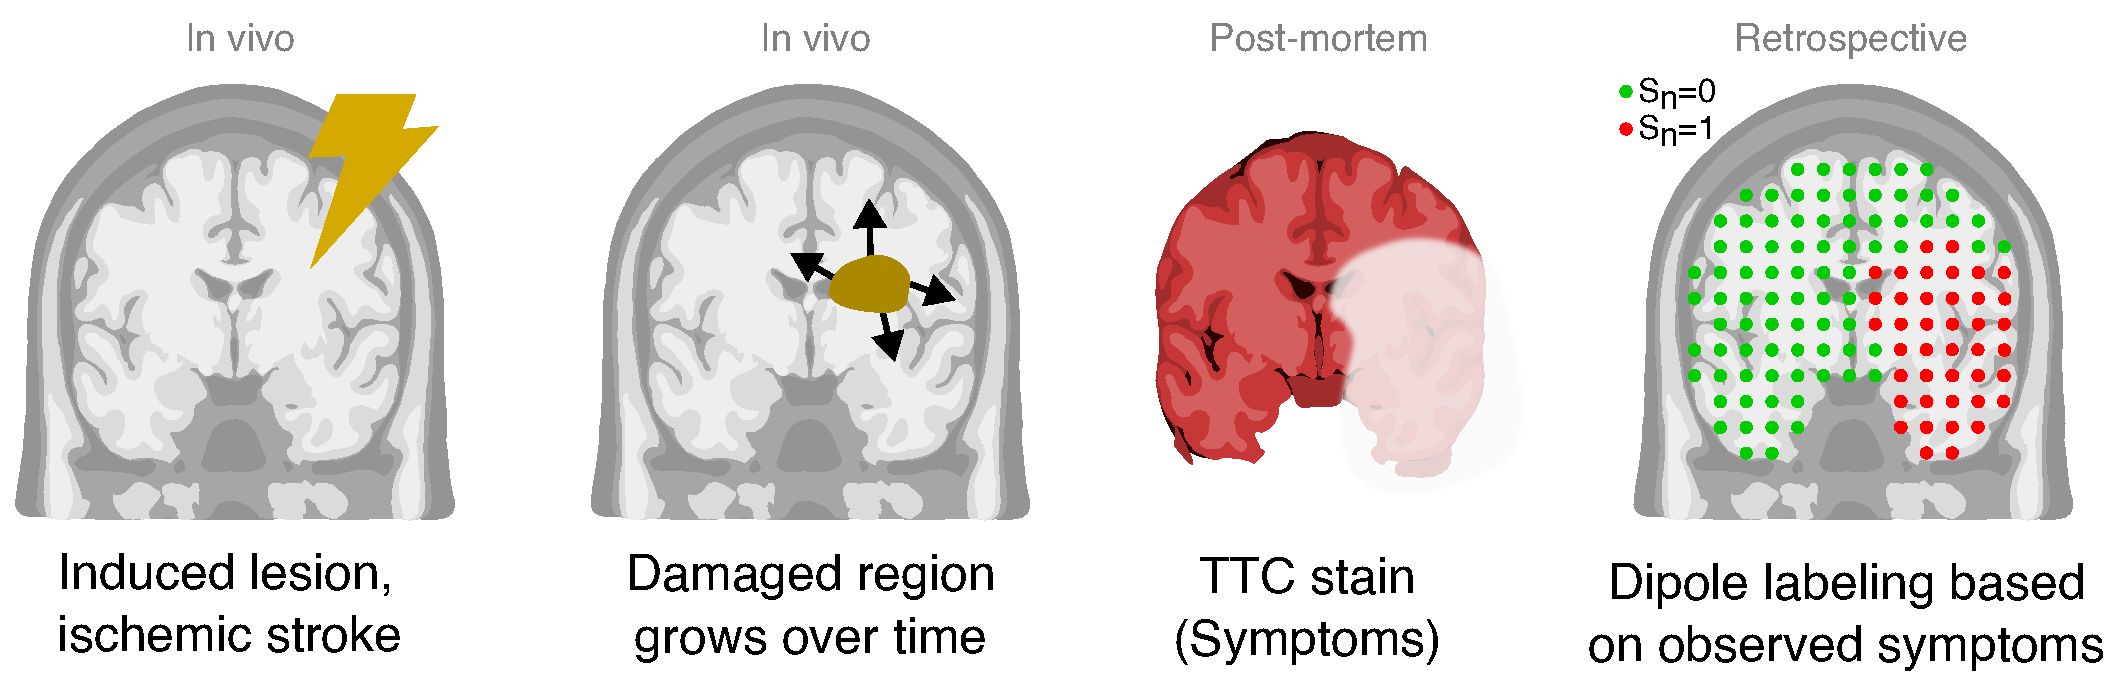
\includegraphics[width=\linewidth]{./img_dev/motivation.pdf}
\caption{This figure is temporary and will be replaced}
\end{figure}

Within the framework of this work, pictures obtained after TTC staining were registered to the template MRI to identify the Ischemic Penumbra at the time of sacrifice.
%
This definition is simplistic and doesn't represent a clinical decision.

The P-region defined in the previous section is determined as the anatomic Ischemic Penumbra observed using TTC stain.





 



 




 


